\section{eSalud}
Teniendo en consideración que el servicio de más alto nivel de la red es la eSalud, es necesario abordar su concepto con el fin de tener un marco para la comprensión del modelo de dominio que se presentará en un capítulo posterior.

La eSalud es definida por la organización Mundial de la Salud (OMS) \cite{oms2016} como \begin{quote}el apoyo que la utilización costo eficaz y segura de las tecnologías de la información y las comunicaciones ofrece a la salud y a los ámbitos relacionados con ella, con inclusión de los servicios de atención de salud, la vigilancia y la documentación sanitarias, así como la educación, los conocimientos y las investigaciones en materia de salud\end{quote}, en si es un término que define un campo multidisciplinar que integra componentes de diferentes áreas del saber que incluye entre otros a la medicina, la ingeniería electrónica, la telemática, la informática, la ingeniería de sistemas, la inteligencia artificial, la biónica, la psicología, la sociología, la antropología, las geociencias, entre muchas otras. Las redes eSalud consideran elementos que van mucho más alla del simple despliegue de redes tecnológicas de intercomunicación y se plantean como redes de interacción social cuyo objetivo primario - más no el único, es la prestación de servicios médicos y relacionados.

Dependiendo el grado en que se presente cada uno de los elementos mostrados en la figura ~\ref{elementosred} y de la mayor o menor correlación entre ellos, se pueden crear sistemas de eSalud que se acerquen al ideal de proveer servicios de salud de alta calidad. 

La OMS y la Unión Internacional de Telecomunicaciones (ITU) proveen \cite{ituoms2012} un método que podría ser utilizado para abordar el desarrollo de proyectos de eSalud complejos, dinámicos y evolutivos. 

\begin{figure}
 \centering
 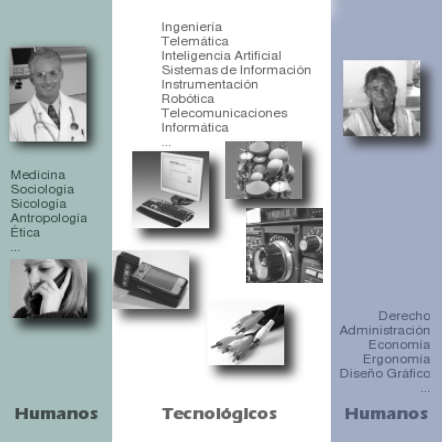
\includegraphics[width=156mm, height=156mm]{sistema_telemedicina.png}
 \caption{Elementos genéricos y áreas del saber de una red de eSalud}
 \label{elementosred}
\end{figure}

\subsection{Componentes Principales de eSalud}

La eSalud comprende áreas que no tienen una división concreta pero se enfocan en ciertos aspectos de interés:

\begin{itemize}
 \item Telemedicina: Provisión remota de servicio clínicos
 \item Telesalud: Telemedicina, complementada con la prestación remota de otros servicios tales como entrenamiento médico, monitoreo de pacientes, cuidado médico, gestión administrativa, etc. 
 \item mSalud: telesalud con el apoyo de dispositivos móviles.
 \item Registro Médico electrónico: Conocido como Historia Clínica Electrónica. Comprende los mecanismos que permiten registrar en un entorno digital seguro, la información sobre los eventos de salud de cada paciente.
 \item eAprendizaje/eEnseñanza: Servicios de enseñanza/aprendizaje de ciencias médica y afines, en modalidad a distancia o virtual.
\end{itemize}

Cabe la pena aclarar que la pluralidad de componentes no es más que un esfuerzo para abordar en un único modelo, todas las tendencias que se han presentado en la evolución de la eSalud. En alguna literatura los términos son intercambiables dependiendo el enfoque del autor. \cite{oms2010}.